\section{Introduction}
Many of the decisions we make are based on recommendation, from either people we know or a recommender system which knows our preferences, due to the amount of information overload we are exposed to. The recommendations, or more specific on our case the recommender system, can be a help to reduce the amount of information we are presented with to a manageable level and hereby ease the decision making without forcing a decision on us. 

The problem with the traditional recommender systems is that it typically make recommendations specifically to one person put often these decisions needs to be taken in a social context. Some scenarios where this could be the case is for example selecting a film to watch from the seemingly endless ones available on the streaming services, Which restaurant you should go to, or which vacation destination suits you best. 

One for the problem regarding taking the social context into consideration is that the recommender have to strive for consensus between the people it recommends to. From here, we will reference to this problem as making a group recommendation.

%Different methods for group recommendations 
When making group recommendations there are two main approach namely profile aggregation and recommendation aggregation.\note{cite, page 516 in rec. book} The idea behind profile aggregation is to aggregate the users preferences into a group profile and make aggregations based on that profile. The recommendation aggregation method aggregates the recommendations for the individual users into one aggregation that should fit the groups preferences. In this paper we have chosen to focus on the latter, as we want to make the method work for shifting groups and we deem this approach to fit this case best. \note{find source or fitting argument}

%Describe the approach of using top-k lists 
As we are going to aggregate the users recommendations we have chosen to only to focus at the top-k part of their recommendations and return a top-k lists as a result. Furthermore, the top-k lists will be ranked with the highest rated item at first position on the list. Throughout the paper we have worked with a $k$ of size 10. 

Working with partial lists, which ranked top-k lists are, we have selected three types of aggregation list which have shown good results when used for aggregating search engine results within the information retrieval domain. The methods we are using is Borda Count, Markov Chain, and Spearman's Footrule. We also implemented an Average aggregation method as a control algorithm. 

%Problem regarding evaluation of the aggregation results
Having the group recommendations we are faced with the challenge of evaluating the result as there are no dataset supplying us with a ground truth. Alternatively we use some different equality measures in order to verify the results. 
\note{extend this}


%Lukas
%As it is no longer of question of should the computers be involved when humans make decisions but how.

%Recommender systems can strengthen decision making without taking away the final choice from humans. This opens the 

%For making a decision, Edwards et al provide a 19 step guide for picking the option with the highest utility, and they argue that the problem for a user would be in picking from among the many options presented, also known as information overload\cite{Edwards2001}.

%Recommender systems deal with reducing the problem for a user to a manageable amount of choices. Given a user's preferences, a good recommender system can narrow down the number of choices to a manageable level.

%However when the problem area is expanded to include multiple users in need of a single choice, the problem area is two-fold, as the many individual preferences must be aligned into that of a single recommendation.

%The recommender system is doubly challenged as while a single user can navigate the given recommendations and reflect on each item for the best optimal choice, a group will have a hard time making insightful decisions about items they lack the shared information of the group to comment on.
\note{Lukas: Possible direction for the introduction?}

\subsection{Composition of a Group Recommender}
As we are going to aggregate recommendations we implemented it as specified in Figure \ref{fig:composition}. Initially we use the dataset to make the individual recommendations and generate the random groups which uses the individual recommendations as a lookup. The next step is where we want to make a contribution and we are trying several different approaches which we evaluate on..
%As we take the aspect of aggregating recommendations the group recommendation system will consist of two parts namely an individual recommender and an aggregation method. \note{need some extension and probably an illustration}
\begin{figure}
\centering
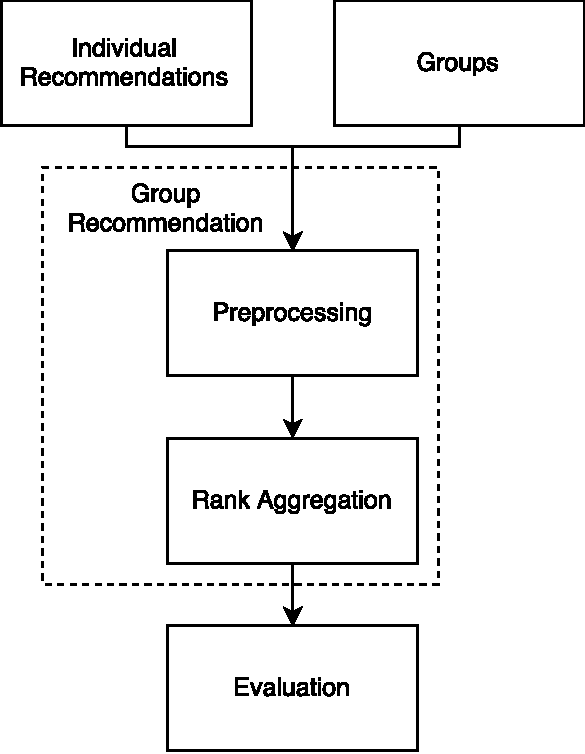
\includegraphics[scale=.4]{graphics/composition}
\caption{Model of the system}\label{fig:composition}
\end{figure}

\subsection{Thesis}\note{Placeholder title}
How can we by supplying a rank aggregation method with an array ranked top-k lists $\tau_1, ... , \tau_u$, where $u$ is the number of group members, get a recommendation performing better than an average aggregation. \note{this should probably be more specific and technical}

\subsection{Structure of the Paper}
The structure of the paper is as follows. In Section \ref{sec:preliminaries} contains the preliminaries including the measures used during the evaluation. Section \ref{sec:aggregations} describes the aggregation methods used. In Section \ref{sec:evaluation} the performances of the aggregation methods are documented. Section \ref{sec:discussion} we discuss the results of the evaluation and in Section \ref{sec:conclusion} we will present our conclusion and some future work to be done.